\section{Algoritmo de Dijkstra}

\begin{frame}[fragile]{Dijkstra $\times$ Bellman-Ford}

    \begin{itemize}
        \item Assim como o algoritmo de Bellman-Ford, o algoritmo de Dijkstra computa as
            distâncias mínimas de todos os vértices $u$ de um grafo $G$ a um nó $s$ dado

        \item Por assumir que todas as arestas não tem peso negativo, este algoritmo tem
            menor complexidade assintótica e pode processar grafos com um maior número de
            nós em relação ao algortimo de Bellman-Ford

        \item Contudo, ele não deve ser usado em grafos ponderados com arestas com pesos
            negativos, pois os resultados produzidos não estarão corretos

        \item A eficiência do algoritmo provém do fato de que cada aresta do grafo é
            processada uma única vez

        \item Isto se dá através de uma escolha inteligente da ordem de processamento dos
            vértices
    \end{itemize}

\end{frame}

\begin{frame}[fragile]{Algoritmo de Dijkstra}

    \begin{itemize}
        \item Inicialmente, a distância de $s$ a $s$ é igual a zero, e todas as demais
            distâncias são iguais a infinito

        \item A cada iteração, o algoritmo escolhe o nó $u$ mais próximo de $s$ que ainda não foi
            processado

        \item Todas as arestas de partem de $u$ então são processadas, atualizando as 
            distâncias quando possível

        \item Esta operação de atualização de distância é chamada relaxamento

        \item Para escolher o próximo nó a ser processado de forma eficiente, é utilizada uma
            fila com prioridade

        \item Desta forma, a complexidade do algortimo é $O(V + E\log E)$

        \item Se o grafo for denso, é possível processar aproximadamente 1.000 vértices

        \item Se o grafo for esparso, é possível computar até um milhão de vértices em
            segundos

    \end{itemize}

\end{frame}

\begin{frame}[fragile]{Visualização do algoritmo de Dijkstra}

    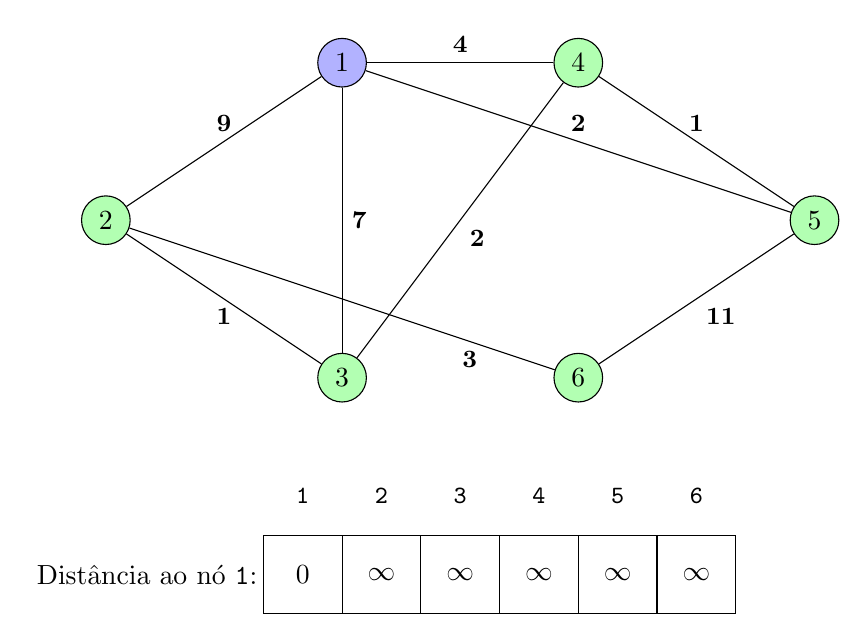
\begin{tikzpicture}
        \node[anchor=west] at (-1, 0.5) { Distância ao nó \texttt{1}: };

        \node[circle, draw, fill=blue!30] (a) at (3, 7) {1};
        \node[circle, draw, fill=green!30] (b) at (0, 5) {2};
        \node[circle, draw, fill=green!30] (c) at (3, 3) {3};
        \node[circle, draw, fill=green!30] (d) at (6, 7) {4};
        \node[circle, draw, fill=green!30] (e) at (9, 5) {5};
        \node[circle, draw, fill=green!30] (f) at (6, 3) {6};

        \draw (2, 0) grid (8, 1);

        \node at (2.5, 0.5) { $0$ };
        \node at (3.5, 0.5) { $\infty$ };
        \node at (4.5, 0.5) { $\infty$ };
        \node at (5.5, 0.5) { $\infty$ };
        \node at (6.5, 0.5) { $\infty$ };
        \node at (7.5, 0.5) { $\infty$ };

        \node at (2.5, 1.5) { \small \texttt{1} };
        \node at (3.5, 1.5) { \small \texttt{2} };
        \node at (4.5, 1.5) { \small \texttt{3} };
        \node at (5.5, 1.5) { \small \texttt{4} };
        \node at (6.5, 1.5) { \small \texttt{5} };
        \node at (7.5, 1.5) { \small \texttt{6} };

        \draw (a) to node[midway,anchor=south] { \small \bfseries 9 } (b);
        \draw (a) to node[midway,anchor=west] { \small \bfseries 7 } (c);
        \draw (a) to node[midway,anchor=south] { \small \bfseries 4 } (d);
        \draw (a) to node[midway,anchor=south] { \small \bfseries 2 } (e);
        \draw (b) to node[midway,anchor=north] { \small \bfseries 1 } (c);
        \draw (b) to node[pos=0.8,anchor=north] { \small \bfseries 3 } (f);
        \draw (c) to node[midway,anchor=north west] { \small \bfseries 2 } (d);
        \draw (d) to node[midway,anchor=south] { \small \bfseries 1 } (e);
        \draw (e) to node[midway,anchor=north west] { \small \bfseries 11 } (f);

    \end{tikzpicture}

\end{frame}

\begin{frame}[fragile]{Visualização do algoritmo de Dijkstra}

    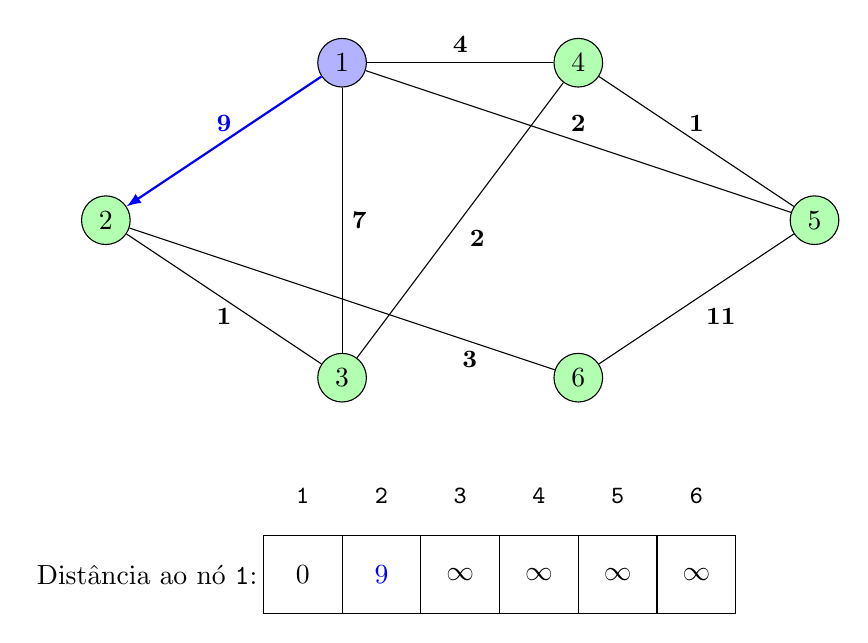
\begin{tikzpicture}
        \node[anchor=west] at (-1, 0.5) { Distância ao nó \texttt{1}: };

        \node[circle, draw, fill=blue!30] (a) at (3, 7) {1};
        \node[circle, draw, fill=green!30] (b) at (0, 5) {2};
        \node[circle, draw, fill=green!30] (c) at (3, 3) {3};
        \node[circle, draw, fill=green!30] (d) at (6, 7) {4};
        \node[circle, draw, fill=green!30] (e) at (9, 5) {5};
        \node[circle, draw, fill=green!30] (f) at (6, 3) {6};

        \draw (2, 0) grid (8, 1);

        \node at (2.5, 0.5) { $0$ };
        \node at (3.5, 0.5) { \textcolor{blue}{$9$} };
        \node at (4.5, 0.5) { $\infty$ };
        \node at (5.5, 0.5) { $\infty$ };
        \node at (6.5, 0.5) { $\infty$ };
        \node at (7.5, 0.5) { $\infty$ };

        \node at (2.5, 1.5) { \small \texttt{1} };
        \node at (3.5, 1.5) { \small \texttt{2} };
        \node at (4.5, 1.5) { \small \texttt{3} };
        \node at (5.5, 1.5) { \small \texttt{4} };
        \node at (6.5, 1.5) { \small \texttt{5} };
        \node at (7.5, 1.5) { \small \texttt{6} };

        %\draw (a) to node[midway,anchor=south] { \small \bfseries 9 } (b);
        \draw[-latex,thick,color=blue] (a) to node[midway,anchor=south] { \small \bfseries 9 } (b);
        \draw (a) to node[midway,anchor=west] { \small \bfseries 7 } (c);
        \draw (a) to node[midway,anchor=south] { \small \bfseries 4 } (d);
        \draw (a) to node[midway,anchor=south] { \small \bfseries 2 } (e);
        \draw (b) to node[midway,anchor=north] { \small \bfseries 1 } (c);
        \draw (b) to node[pos=0.8,anchor=north] { \small \bfseries 3 } (f);
        \draw (c) to node[midway,anchor=north west] { \small \bfseries 2 } (d);
        \draw (d) to node[midway,anchor=south] { \small \bfseries 1 } (e);
        \draw (e) to node[midway,anchor=north west] { \small \bfseries 11 } (f);

    \end{tikzpicture}

\end{frame}

\begin{frame}[fragile]{Visualização do algoritmo de Dijkstra}

    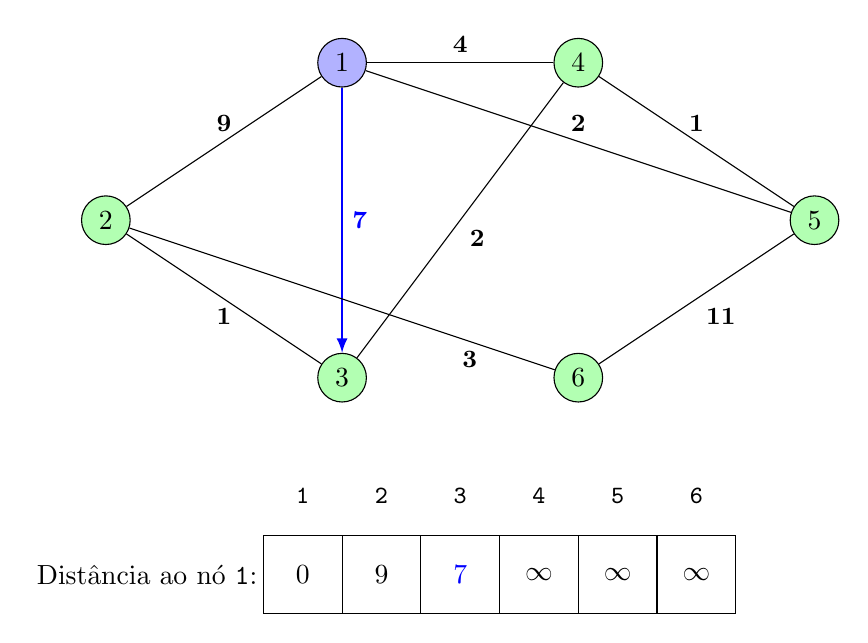
\begin{tikzpicture}
        \node[anchor=west] at (-1, 0.5) { Distância ao nó \texttt{1}: };

        \node[circle, draw, fill=blue!30] (a) at (3, 7) {1};
        \node[circle, draw, fill=green!30] (b) at (0, 5) {2};
        \node[circle, draw, fill=green!30] (c) at (3, 3) {3};
        \node[circle, draw, fill=green!30] (d) at (6, 7) {4};
        \node[circle, draw, fill=green!30] (e) at (9, 5) {5};
        \node[circle, draw, fill=green!30] (f) at (6, 3) {6};

        \draw (2, 0) grid (8, 1);

        \node at (2.5, 0.5) { $0$ };
        \node at (3.5, 0.5) { \textcolor{black}{$9$} };
        \node at (4.5, 0.5) { \textcolor{blue}{$7$} };
        \node at (5.5, 0.5) { $\infty$ };
        \node at (6.5, 0.5) { $\infty$ };
        \node at (7.5, 0.5) { $\infty$ };

        \node at (2.5, 1.5) { \small \texttt{1} };
        \node at (3.5, 1.5) { \small \texttt{2} };
        \node at (4.5, 1.5) { \small \texttt{3} };
        \node at (5.5, 1.5) { \small \texttt{4} };
        \node at (6.5, 1.5) { \small \texttt{5} };
        \node at (7.5, 1.5) { \small \texttt{6} };

        \draw (a) to node[midway,anchor=south] { \small \bfseries 9 } (b);
        %\draw (a) to node[midway,anchor=west] { \small \bfseries 7 } (c);
        \draw[-latex,thick,color=blue] (a) to node[midway,anchor=west] { \small \bfseries 7 } (c);
        \draw (a) to node[midway,anchor=south] { \small \bfseries 4 } (d);
        \draw (a) to node[midway,anchor=south] { \small \bfseries 2 } (e);
        \draw (b) to node[midway,anchor=north] { \small \bfseries 1 } (c);
        \draw (b) to node[pos=0.8,anchor=north] { \small \bfseries 3 } (f);
        \draw (c) to node[midway,anchor=north west] { \small \bfseries 2 } (d);
        \draw (d) to node[midway,anchor=south] { \small \bfseries 1 } (e);
        \draw (e) to node[midway,anchor=north west] { \small \bfseries 11 } (f);

    \end{tikzpicture}

\end{frame}

\begin{frame}[fragile]{Visualização do algoritmo de Dijkstra}

    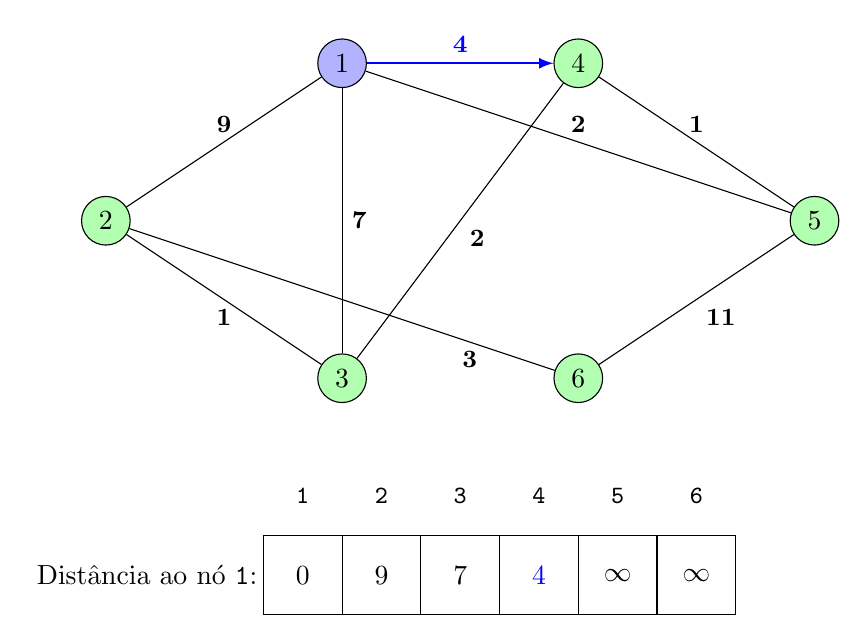
\begin{tikzpicture}
        \node[anchor=west] at (-1, 0.5) { Distância ao nó \texttt{1}: };

        \node[circle, draw, fill=blue!30] (a) at (3, 7) {1};
        \node[circle, draw, fill=green!30] (b) at (0, 5) {2};
        \node[circle, draw, fill=green!30] (c) at (3, 3) {3};
        \node[circle, draw, fill=green!30] (d) at (6, 7) {4};
        \node[circle, draw, fill=green!30] (e) at (9, 5) {5};
        \node[circle, draw, fill=green!30] (f) at (6, 3) {6};

        \draw (2, 0) grid (8, 1);

        \node at (2.5, 0.5) { $0$ };
        \node at (3.5, 0.5) { \textcolor{black}{$9$} };
        \node at (4.5, 0.5) { \textcolor{black}{$7$} };
        \node at (5.5, 0.5) { \textcolor{blue}{$4$} };
        \node at (6.5, 0.5) { $\infty$ };
        \node at (7.5, 0.5) { $\infty$ };

        \node at (2.5, 1.5) { \small \texttt{1} };
        \node at (3.5, 1.5) { \small \texttt{2} };
        \node at (4.5, 1.5) { \small \texttt{3} };
        \node at (5.5, 1.5) { \small \texttt{4} };
        \node at (6.5, 1.5) { \small \texttt{5} };
        \node at (7.5, 1.5) { \small \texttt{6} };

        \draw (a) to node[midway,anchor=south] { \small \bfseries 9 } (b);
        \draw (a) to node[midway,anchor=west] { \small \bfseries 7 } (c);
        %\draw (a) to node[midway,anchor=south] { \small \bfseries 4 } (d);
        \draw[-latex,thick,blue] (a) to node[midway,anchor=south] { \small \bfseries 4 } (d);
        \draw (a) to node[midway,anchor=south] { \small \bfseries 2 } (e);
        \draw (b) to node[midway,anchor=north] { \small \bfseries 1 } (c);
        \draw (b) to node[pos=0.8,anchor=north] { \small \bfseries 3 } (f);
        \draw (c) to node[midway,anchor=north west] { \small \bfseries 2 } (d);
        \draw (d) to node[midway,anchor=south] { \small \bfseries 1 } (e);
        \draw (e) to node[midway,anchor=north west] { \small \bfseries 11 } (f);

    \end{tikzpicture}

\end{frame}

\begin{frame}[fragile]{Visualização do algoritmo de Dijkstra}

    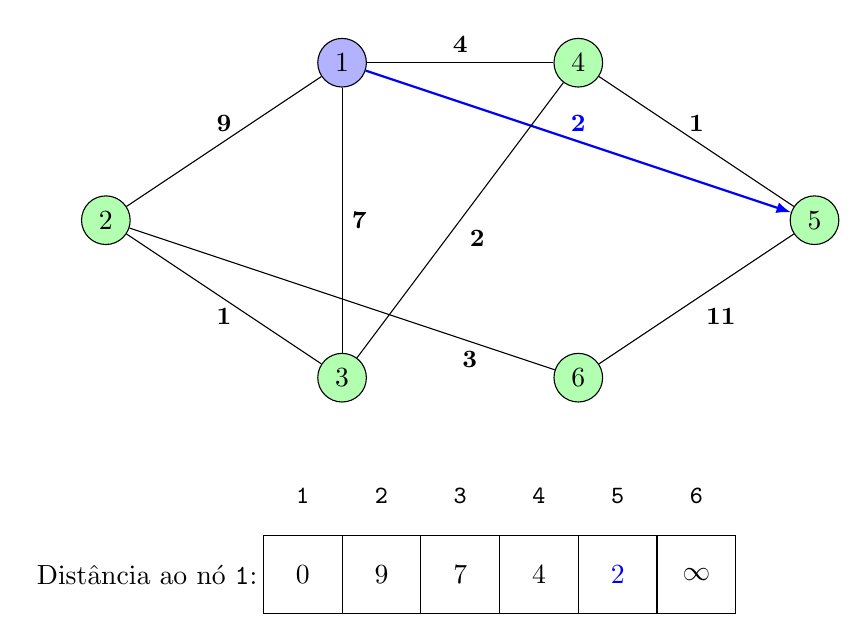
\begin{tikzpicture}
        \node[anchor=west] at (-1, 0.5) { Distância ao nó \texttt{1}: };

        \node[circle, draw, fill=blue!30] (a) at (3, 7) {1};
        \node[circle, draw, fill=green!30] (b) at (0, 5) {2};
        \node[circle, draw, fill=green!30] (c) at (3, 3) {3};
        \node[circle, draw, fill=green!30] (d) at (6, 7) {4};
        \node[circle, draw, fill=green!30] (e) at (9, 5) {5};
        \node[circle, draw, fill=green!30] (f) at (6, 3) {6};

        \draw (2, 0) grid (8, 1);

        \node at (2.5, 0.5) { $0$ };
        \node at (3.5, 0.5) { \textcolor{black}{$9$} };
        \node at (4.5, 0.5) { \textcolor{black}{$7$} };
        \node at (5.5, 0.5) { \textcolor{black}{$4$} };
        \node at (6.5, 0.5) { \textcolor{blue}{$2$} };
        \node at (7.5, 0.5) { $\infty$ };

        \node at (2.5, 1.5) { \small \texttt{1} };
        \node at (3.5, 1.5) { \small \texttt{2} };
        \node at (4.5, 1.5) { \small \texttt{3} };
        \node at (5.5, 1.5) { \small \texttt{4} };
        \node at (6.5, 1.5) { \small \texttt{5} };
        \node at (7.5, 1.5) { \small \texttt{6} };

        \draw (a) to node[midway,anchor=south] { \small \bfseries 9 } (b);
        \draw (a) to node[midway,anchor=west] { \small \bfseries 7 } (c);
        \draw (a) to node[midway,anchor=south] { \small \bfseries 4 } (d);
        %\draw (a) to node[midway,anchor=south] { \small \bfseries 2 } (e);
        \draw[-latex,thick,blue] (a) to node[midway,anchor=south] { \small \bfseries 2 } (e);
        \draw (b) to node[midway,anchor=north] { \small \bfseries 1 } (c);
        \draw (b) to node[pos=0.8,anchor=north] { \small \bfseries 3 } (f);
        \draw (c) to node[midway,anchor=north west] { \small \bfseries 2 } (d);
        \draw (d) to node[midway,anchor=south] { \small \bfseries 1 } (e);
        \draw (e) to node[midway,anchor=north west] { \small \bfseries 11 } (f);

    \end{tikzpicture}

\end{frame}

\begin{frame}[fragile]{Visualização do algoritmo de Dijkstra}

    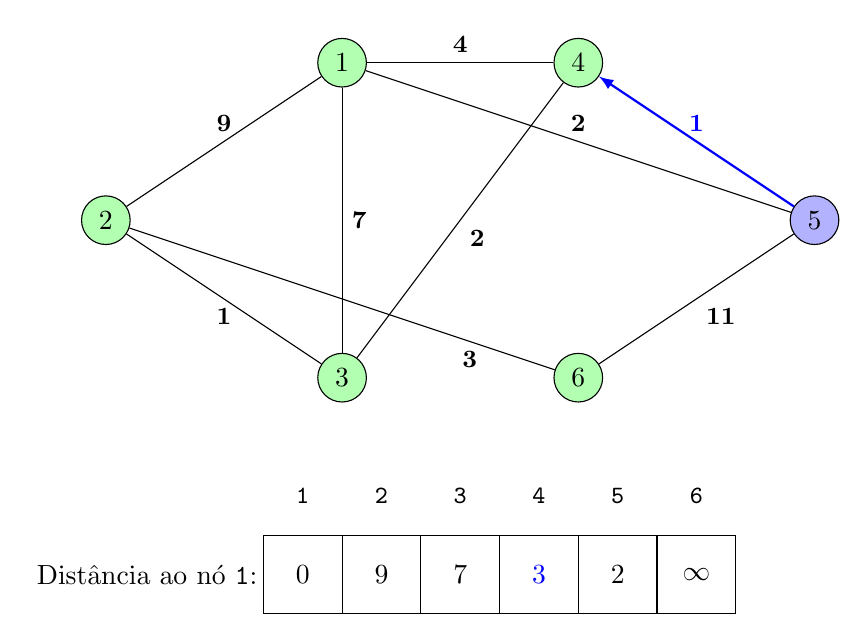
\begin{tikzpicture}
        \node[anchor=west] at (-1, 0.5) { Distância ao nó \texttt{1}: };

        \node[circle, draw, fill=green!30] (a) at (3, 7) {1};
        \node[circle, draw, fill=green!30] (b) at (0, 5) {2};
        \node[circle, draw, fill=green!30] (c) at (3, 3) {3};
        \node[circle, draw, fill=green!30] (d) at (6, 7) {4};
        \node[circle, draw, fill=blue!30] (e) at (9, 5) {5};
        \node[circle, draw, fill=green!30] (f) at (6, 3) {6};

        \draw (2, 0) grid (8, 1);

        \node at (2.5, 0.5) { $0$ };
        \node at (3.5, 0.5) { \textcolor{black}{$9$} };
        \node at (4.5, 0.5) { \textcolor{black}{$7$} };
        \node at (5.5, 0.5) { \textcolor{blue}{$3$} };
        \node at (6.5, 0.5) { \textcolor{black}{$2$} };
        \node at (7.5, 0.5) { $\infty$ };

        \node at (2.5, 1.5) { \small \texttt{1} };
        \node at (3.5, 1.5) { \small \texttt{2} };
        \node at (4.5, 1.5) { \small \texttt{3} };
        \node at (5.5, 1.5) { \small \texttt{4} };
        \node at (6.5, 1.5) { \small \texttt{5} };
        \node at (7.5, 1.5) { \small \texttt{6} };

        \draw (a) to node[midway,anchor=south] { \small \bfseries 9 } (b);
        \draw (a) to node[midway,anchor=west] { \small \bfseries 7 } (c);
        \draw (a) to node[midway,anchor=south] { \small \bfseries 4 } (d);
        \draw (a) to node[midway,anchor=south] { \small \bfseries 2 } (e);
        \draw (b) to node[midway,anchor=north] { \small \bfseries 1 } (c);
        \draw (b) to node[pos=0.8,anchor=north] { \small \bfseries 3 } (f);
        \draw (c) to node[midway,anchor=north west] { \small \bfseries 2 } (d);
        %\draw (d) to node[midway,anchor=south] { \small \bfseries 1 } (e);
        \draw[latex-,thick,blue] (d) to node[midway,anchor=south] { \small \bfseries 1 } (e);
        \draw (e) to node[midway,anchor=north west] { \small \bfseries 11 } (f);

    \end{tikzpicture}

\end{frame}

\begin{frame}[fragile]{Visualização do algoritmo de Dijkstra}

    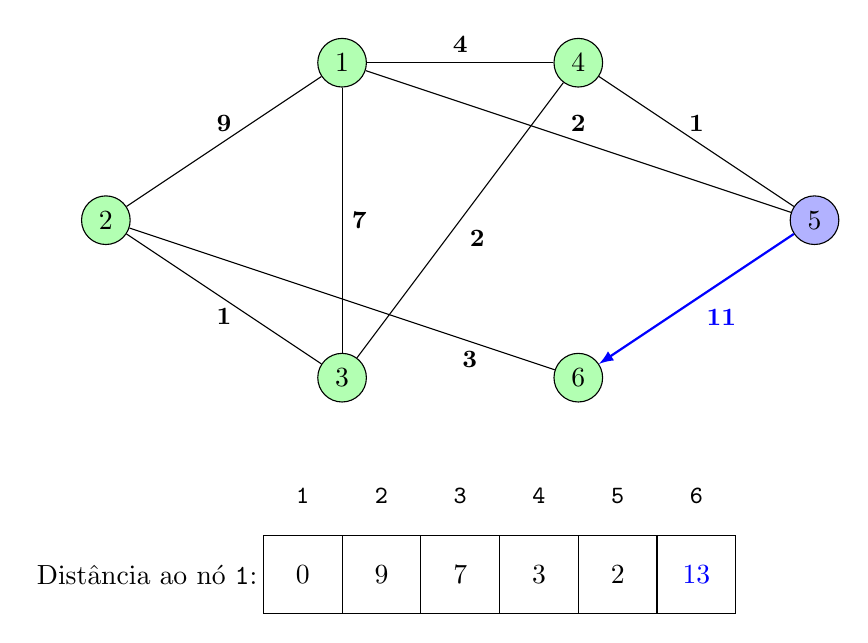
\begin{tikzpicture}
        \node[anchor=west] at (-1, 0.5) { Distância ao nó \texttt{1}: };

        \node[circle, draw, fill=green!30] (a) at (3, 7) {1};
        \node[circle, draw, fill=green!30] (b) at (0, 5) {2};
        \node[circle, draw, fill=green!30] (c) at (3, 3) {3};
        \node[circle, draw, fill=green!30] (d) at (6, 7) {4};
        \node[circle, draw, fill=blue!30] (e) at (9, 5) {5};
        \node[circle, draw, fill=green!30] (f) at (6, 3) {6};

        \draw (2, 0) grid (8, 1);

        \node at (2.5, 0.5) { $0$ };
        \node at (3.5, 0.5) { \textcolor{black}{$9$} };
        \node at (4.5, 0.5) { \textcolor{black}{$7$} };
        \node at (5.5, 0.5) { \textcolor{black}{$3$} };
        \node at (6.5, 0.5) { \textcolor{black}{$2$} };
        \node at (7.5, 0.5) { \textcolor{blue}{$13$} };

        \node at (2.5, 1.5) { \small \texttt{1} };
        \node at (3.5, 1.5) { \small \texttt{2} };
        \node at (4.5, 1.5) { \small \texttt{3} };
        \node at (5.5, 1.5) { \small \texttt{4} };
        \node at (6.5, 1.5) { \small \texttt{5} };
        \node at (7.5, 1.5) { \small \texttt{6} };

        \draw (a) to node[midway,anchor=south] { \small \bfseries 9 } (b);
        \draw (a) to node[midway,anchor=west] { \small \bfseries 7 } (c);
        \draw (a) to node[midway,anchor=south] { \small \bfseries 4 } (d);
        \draw (a) to node[midway,anchor=south] { \small \bfseries 2 } (e);
        \draw (b) to node[midway,anchor=north] { \small \bfseries 1 } (c);
        \draw (b) to node[pos=0.8,anchor=north] { \small \bfseries 3 } (f);
        \draw (c) to node[midway,anchor=north west] { \small \bfseries 2 } (d);
        \draw (d) to node[midway,anchor=south] { \small \bfseries 1 } (e);
        %\draw (e) to node[midway,anchor=north west] { \small \bfseries 11 } (f);
        \draw[-latex,thick,blue] (e) to node[midway,anchor=north west] { \small \bfseries 11 } (f);

    \end{tikzpicture}

\end{frame}

\begin{frame}[fragile]{Visualização do algoritmo de Dijkstra}

    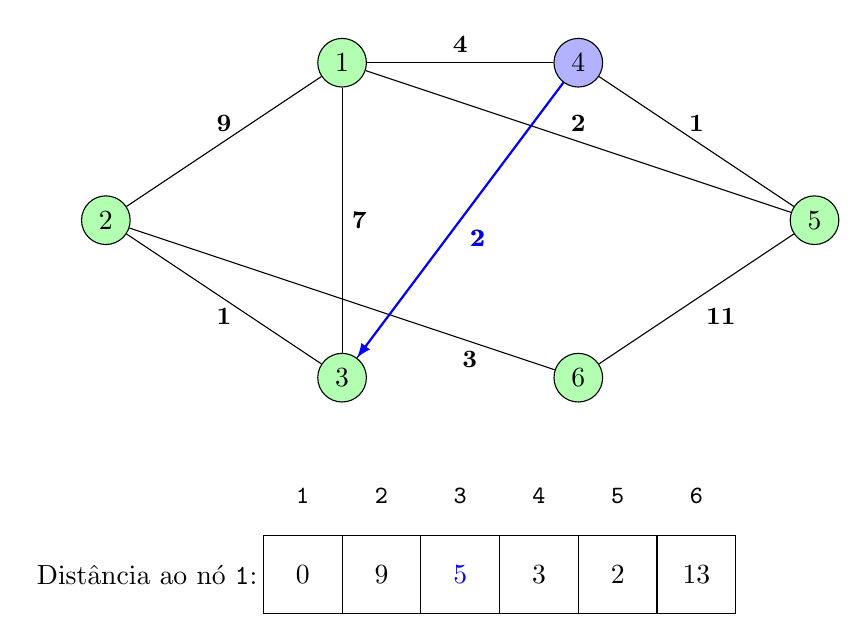
\begin{tikzpicture}
        \node[anchor=west] at (-1, 0.5) { Distância ao nó \texttt{1}: };

        \node[circle, draw, fill=green!30] (a) at (3, 7) {1};
        \node[circle, draw, fill=green!30] (b) at (0, 5) {2};
        \node[circle, draw, fill=green!30] (c) at (3, 3) {3};
        \node[circle, draw, fill=blue!30] (d) at (6, 7) {4};
        \node[circle, draw, fill=green!30] (e) at (9, 5) {5};
        \node[circle, draw, fill=green!30] (f) at (6, 3) {6};

        \draw (2, 0) grid (8, 1);

        \node at (2.5, 0.5) { $0$ };
        \node at (3.5, 0.5) { \textcolor{black}{$9$} };
        \node at (4.5, 0.5) { \textcolor{blue}{$5$} };
        \node at (5.5, 0.5) { \textcolor{black}{$3$} };
        \node at (6.5, 0.5) { \textcolor{black}{$2$} };
        \node at (7.5, 0.5) { \textcolor{black}{$13$} };

        \node at (2.5, 1.5) { \small \texttt{1} };
        \node at (3.5, 1.5) { \small \texttt{2} };
        \node at (4.5, 1.5) { \small \texttt{3} };
        \node at (5.5, 1.5) { \small \texttt{4} };
        \node at (6.5, 1.5) { \small \texttt{5} };
        \node at (7.5, 1.5) { \small \texttt{6} };

        \draw (a) to node[midway,anchor=south] { \small \bfseries 9 } (b);
        \draw (a) to node[midway,anchor=west] { \small \bfseries 7 } (c);
        \draw (a) to node[midway,anchor=south] { \small \bfseries 4 } (d);
        \draw (a) to node[midway,anchor=south] { \small \bfseries 2 } (e);
        \draw (b) to node[midway,anchor=north] { \small \bfseries 1 } (c);
        \draw (b) to node[pos=0.8,anchor=north] { \small \bfseries 3 } (f);
        \draw (c) to node[midway,anchor=north west] { \small \bfseries 2 } (d);
        \draw[latex-,thick,blue] (c) to node[midway,anchor=north west] { \small \bfseries 2 } (d);
        \draw (d) to node[midway,anchor=south] { \small \bfseries 1 } (e);
        \draw (e) to node[midway,anchor=north west] { \small \bfseries 11 } (f);

    \end{tikzpicture}

\end{frame}

\begin{frame}[fragile]{Visualização do algoritmo de Dijkstra}

    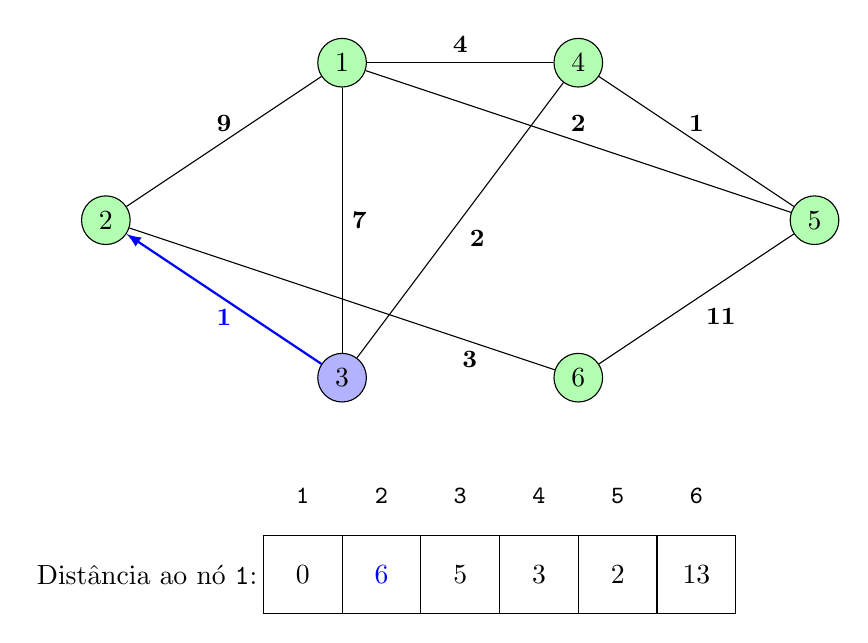
\begin{tikzpicture}
        \node[anchor=west] at (-1, 0.5) { Distância ao nó \texttt{1}: };

        \node[circle, draw, fill=green!30] (a) at (3, 7) {1};
        \node[circle, draw, fill=green!30] (b) at (0, 5) {2};
        \node[circle, draw, fill=blue!30] (c) at (3, 3) {3};
        \node[circle, draw, fill=green!30] (d) at (6, 7) {4};
        \node[circle, draw, fill=green!30] (e) at (9, 5) {5};
        \node[circle, draw, fill=green!30] (f) at (6, 3) {6};

        \draw (2, 0) grid (8, 1);

        \node at (2.5, 0.5) { $0$ };
        \node at (3.5, 0.5) { \textcolor{blue}{$6$} };
        \node at (4.5, 0.5) { \textcolor{black}{$5$} };
        \node at (5.5, 0.5) { \textcolor{black}{$3$} };
        \node at (6.5, 0.5) { \textcolor{black}{$2$} };
        \node at (7.5, 0.5) { \textcolor{black}{$13$} };

        \node at (2.5, 1.5) { \small \texttt{1} };
        \node at (3.5, 1.5) { \small \texttt{2} };
        \node at (4.5, 1.5) { \small \texttt{3} };
        \node at (5.5, 1.5) { \small \texttt{4} };
        \node at (6.5, 1.5) { \small \texttt{5} };
        \node at (7.5, 1.5) { \small \texttt{6} };

        \draw (a) to node[midway,anchor=south] { \small \bfseries 9 } (b);
        \draw (a) to node[midway,anchor=west] { \small \bfseries 7 } (c);
        \draw (a) to node[midway,anchor=south] { \small \bfseries 4 } (d);
        \draw (a) to node[midway,anchor=south] { \small \bfseries 2 } (e);
        %\draw (b) to node[midway,anchor=north] { \small \bfseries 1 } (c);
        \draw[latex-,thick,blue] (b) to node[midway,anchor=north] { \small \bfseries 1 } (c);
        \draw (b) to node[pos=0.8,anchor=north] { \small \bfseries 3 } (f);
        \draw (c) to node[midway,anchor=north west] { \small \bfseries 2 } (d);
        \draw (d) to node[midway,anchor=south] { \small \bfseries 1 } (e);
        \draw (e) to node[midway,anchor=north west] { \small \bfseries 11 } (f);

    \end{tikzpicture}

\end{frame}

\begin{frame}[fragile]{Visualização do algoritmo de Dijkstra}

    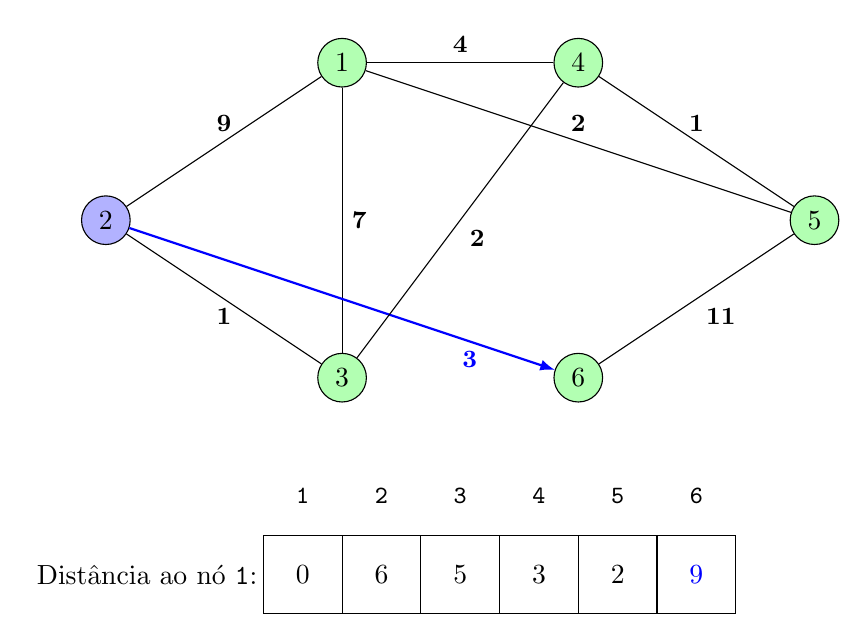
\begin{tikzpicture}
        \node[anchor=west] at (-1, 0.5) { Distância ao nó \texttt{1}: };

        \node[circle, draw, fill=green!30] (a) at (3, 7) {1};
        \node[circle, draw, fill=blue!30] (b) at (0, 5) {2};
        \node[circle, draw, fill=green!30] (c) at (3, 3) {3};
        \node[circle, draw, fill=green!30] (d) at (6, 7) {4};
        \node[circle, draw, fill=green!30] (e) at (9, 5) {5};
        \node[circle, draw, fill=green!30] (f) at (6, 3) {6};

        \draw (2, 0) grid (8, 1);

        \node at (2.5, 0.5) { $0$ };
        \node at (3.5, 0.5) { \textcolor{black}{$6$} };
        \node at (4.5, 0.5) { \textcolor{black}{$5$} };
        \node at (5.5, 0.5) { \textcolor{black}{$3$} };
        \node at (6.5, 0.5) { \textcolor{black}{$2$} };
        \node at (7.5, 0.5) { \textcolor{blue}{$9$} };

        \node at (2.5, 1.5) { \small \texttt{1} };
        \node at (3.5, 1.5) { \small \texttt{2} };
        \node at (4.5, 1.5) { \small \texttt{3} };
        \node at (5.5, 1.5) { \small \texttt{4} };
        \node at (6.5, 1.5) { \small \texttt{5} };
        \node at (7.5, 1.5) { \small \texttt{6} };

        \draw (a) to node[midway,anchor=south] { \small \bfseries 9 } (b);
        \draw (a) to node[midway,anchor=west] { \small \bfseries 7 } (c);
        \draw (a) to node[midway,anchor=south] { \small \bfseries 4 } (d);
        \draw (a) to node[midway,anchor=south] { \small \bfseries 2 } (e);
        \draw (b) to node[midway,anchor=north] { \small \bfseries 1 } (c);
        %\draw (b) to node[pos=0.8,anchor=north] { \small \bfseries 3 } (f);
        \draw[-latex,thick,blue] (b) to node[pos=0.8,anchor=north] { \small \bfseries 3 } (f);
        \draw (c) to node[midway,anchor=north west] { \small \bfseries 2 } (d);
        \draw (d) to node[midway,anchor=south] { \small \bfseries 1 } (e);
        \draw (e) to node[midway,anchor=north west] { \small \bfseries 11 } (f);

    \end{tikzpicture}

\end{frame}

\begin{frame}[fragile]{Implementação do algoritmo de Dijkstra em C++}
    \inputsnippet{c++}{1}{21}{dijkstra.cpp}
\end{frame}

\begin{frame}[fragile]{Implementação do algoritmo de Dijkstra em C++}
    \inputsnippet{c++}{22}{42}{dijkstra.cpp}
\end{frame}

\begin{frame}[fragile]{Implementação do algoritmo de Dijkstra em C++}
    \inputsnippet{c++}{43}{63}{dijkstra.cpp}
\end{frame}

\section{Caminhos mínimos}


\begin{frame}[fragile]{Identificação do caminho mínimo}

    \begin{itemize}
        \item Assim como no algoritmo de Bellman-Ford, é possível recuperar a sequência de 
            arestas que compõem o caminho mínimo

        \item Para determinar o caminho, é preciso manter o vetor \code{c++}{pred}, onde
            \code{c++}{pred[u]} é o nó que antecede $u$ no caminho mínimo que vai de $s$ a 
            $u$

        \item Inicialmente, todos os elementos deste vetor devem ser iguais a um valor sentinela,
            exceto o vértice $s$, que terá \code{c++}{pred[s] = s}

        \item Se a aresta $(u, v)$ atualizar a distância \code{c++}{dist[v]}, então o 
            predecessor deve ser atualizado também: \code{c++}{pred[v] = u}

        \item Deste modo, o caminho pode ser recuperado, passando por todos os predecessores até
            se atingir o nó $s$

        \item Se o predecessor de $u$ for o valor sentinela, não há caminho de $s$ a $u$ no
            grafo
    \end{itemize}

\end{frame}

\begin{frame}[fragile]{Recuperação do caminho mínimo}
    \inputsnippet{c++}{1}{21}{dijkstra2.cpp}
\end{frame}

\begin{frame}[fragile]{Recuperação do caminho mínimo}
    \inputsnippet{c++}{22}{42}{dijkstra2.cpp}
\end{frame}

\begin{frame}[fragile]{Recuperação do caminho mínimo}
    \inputsnippet{c++}{43}{63}{dijkstra2.cpp}
\end{frame}

\begin{frame}[fragile]{Recuperação do caminho mínimo}
    \inputsnippet{c++}{64}{84}{dijkstra2.cpp}
\end{frame}
